\documentclass[12pt,a4paper]{article}
\usepackage[utf8]{inputenc}
\usepackage[T5]{fontenc}
\usepackage{graphicx}
\usepackage{hyperref}
\usepackage{geometry}
\geometry{top=2.5cm, bottom=2.5cm, left=2.5cm, right=2.5cm}
\usepackage{tikz}
\usetikzlibrary{positioning, shapes.multipart, arrows.meta}

\renewcommand{\figurename}{Hình}
\usepackage[labelsep=none]{caption}
\makeatletter
\setlength{\@fptop}{0pt}
\setlength{\@fpbot}{0pt plus 1fil}
\makeatother

\title{\vspace*{2cm}\huge\textbf{Báo cáo thực hành 03}}
\author{\Large Mã sinh viên: 202418834 \\ \Large Họ tên: Trần Tuấn Anh}
\date{\today}

\begin{document}

\maketitle

\section{Mô tả bài toán}
Bài toán yêu cầu xây dựng chương trình quản lý các nhóm dự án và nhân sự trong một công ty. Nhân sự bao gồm hai loại: nhân sự thông thường (\textbf{Employee}) và kỹ sư phần mềm (\textbf{SoftwareEngineer} - có thêm ngôn ngữ chính và phụ cấp). Mỗi nhóm dự án (\textbf{ProjectTeam}) có một trưởng nhóm và một danh sách các thành viên. Trưởng nhóm cũng là một nhân sự được phân công nhưng không xuất hiện hai lần trong danh sách thành viên của nhóm. 

Yêu cầu hệ thống cần:
\begin{itemize}
    \item Đảm bảo các bất biến: Mã nhân sự không rỗng, lương không âm, nhân sự không trùng lặp trong một nhóm.
    \item Ứng dụng tính đa hình trong việc tính chi phí lương hằng tháng và hiển thị thông tin.
    \item Thể hiện rõ quan hệ kế thừa và quan hệ kết tập (Aggregation).
\end{itemize}

\newpage
\section{Sơ đồ thiết kế (Class Diagram)}

\begin{center}
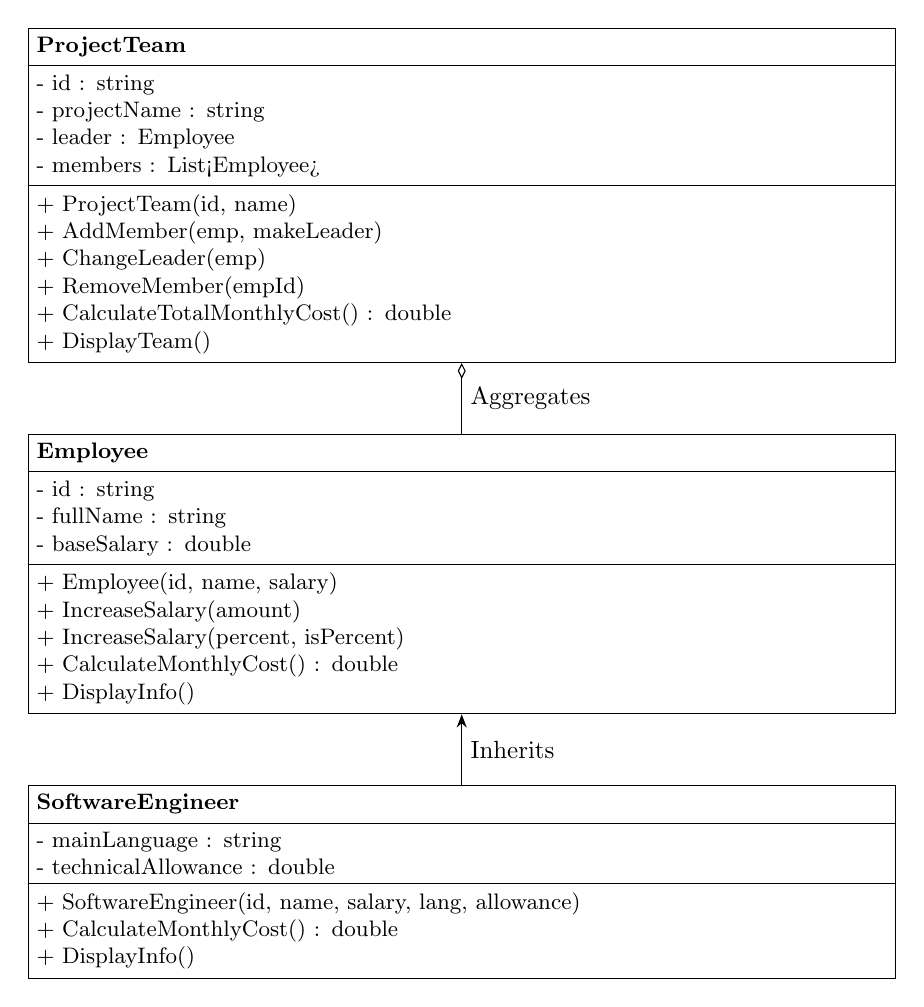
\begin{tikzpicture}[
  transform shape,
  scale=0.9,
  class/.style={
    draw,
    rectangle split,
    rectangle split parts=3,
    text width=12cm,
    font=\small
  },
  >=Stealth,
  node distance=1cm
]

% ProjectTeam
\node[class] (ProjectTeam) {
  \textbf{ProjectTeam}
  \nodepart{two}
  - id : string\\
  - projectName : string\\
  - leader : Employee\\
  - members : List<Employee>
  \nodepart{three}
  + ProjectTeam(id, name)\\
  + AddMember(emp, makeLeader)\\
  + ChangeLeader(emp)\\
  + RemoveMember(empId)\\
  + CalculateTotalMonthlyCost() : double\\
  + DisplayTeam()
};

% Employee
\node[class, below=of ProjectTeam] (Employee) {
  \textbf{Employee}
  \nodepart{two}
  - id : string\\
  - fullName : string\\
  - baseSalary : double
  \nodepart{three}
  + Employee(id, name, salary)\\
  + IncreaseSalary(amount)\\
  + IncreaseSalary(percent, isPercent)\\
  + CalculateMonthlyCost() : double\\
  + DisplayInfo()
};

% SoftwareEngineer
\node[class, below=of Employee] (SoftwareEngineer) {
  \textbf{SoftwareEngineer}
  \nodepart{two}
  - mainLanguage : string\\
  - technicalAllowance : double
  \nodepart{three}
  + SoftwareEngineer(id, name, salary, lang, allowance)\\
  + CalculateMonthlyCost() : double\\
  + DisplayInfo()
};

% Relationships
\draw[->] (SoftwareEngineer.north) -- (Employee.south) node[midway, right] {Inherits};
\draw[{Diamond[open]}-] (ProjectTeam.south) -- (Employee.north) node[midway, right] {Aggregates};

\end{tikzpicture}
\end{center}

\newpage
\section{Mã nguồn khái quát}
Mã nguồn được lập trình bằng ngôn ngữ C\#, phân bổ thành các file lớp độc lập: \texttt{Employee.cs}, \texttt{SoftwareEngineer.cs}, \texttt{ProjectTeam.cs} dựa trên biểu diễn của sơ đồ UML. File \texttt{Program.cs} chứa khối lệnh thực thi kịch bản kiểm thử với đầy đủ 15 bước yêu cầu để kiểm chứng tính đa hình và quản lý vòng đời đối tượng.

Toàn bộ mã nguồn hoàn chỉnh được lưu trữ và có thể truy cập tại Github:
\vspace{0.2cm}

\textbf{Link Github:} \url{https://github.com/tuananhtran109/OOP-Ex03}

\vspace{0.5cm}

\section{Kết quả chạy thử chương trình}

\begin{figure}[htbp]
    \centering
    \includegraphics[width=0.9\textwidth]{test_img_1}
    \caption{}
\end{figure}

\begin{figure}[htbp]
    \centering
    \includegraphics[width=0.9\textwidth]{test_img_2}
    \caption{}
\end{figure}

\begin{figure}[htbp]
    \centering
    \includegraphics[width=0.9\textwidth]{test_img_3}
    \caption{}
\end{figure}

\begin{figure}[htbp]
    \centering
    \includegraphics[width=0.9\textwidth]{test_img_4}
    \caption{}
\end{figure}

\begin{figure}[htbp]
    \centering
    \includegraphics[width=0.9\textwidth]{test_img_5}
    \caption{}
\end{figure}

\begin{figure}[htbp]
    \centering
    \includegraphics[width=0.9\textwidth]{test_img_6}
    \caption{}
\end{figure}

\begin{figure}[htbp]
    \centering
    \includegraphics[width=0.9\textwidth]{test_img_7}
    \caption{}
\end{figure}

\begin{figure}[htbp]
    \centering
    \includegraphics[width=0.9\textwidth]{test_img_8}
    \caption{}
\end{figure}

\begin{figure}[htbp]
    \centering
    \includegraphics[width=0.9\textwidth]{test_img_9}
    \caption{}
\end{figure}

\begin{figure}[htbp]
    \centering
    \includegraphics[width=0.9\textwidth]{test_img_10}
    \caption{}
\end{figure}

\begin{figure}[htbp]
    \centering
    \includegraphics[width=0.9\textwidth]{test_img_11}
    \caption{}
\end{figure}

\begin{figure}[htbp]
    \centering
    \includegraphics[width=0.9\textwidth]{test_img_12}
    \caption{}
\end{figure}

\begin{figure}[htbp]
    \centering
    \includegraphics[width=0.9\textwidth]{test_img_13}
    \caption{}
\end{figure}

\begin{figure}[htbp]
    \centering
    \includegraphics[width=0.9\textwidth]{test_img_14}
    \caption{}
\end{figure}

\begin{figure}[htbp]
    \centering
    \includegraphics[width=0.9\textwidth]{test_img_15}
    \caption{}
\end{figure}

\begin{figure}[htbp]
    \centering
    \includegraphics[width=0.9\textwidth]{test_img_16}
    \caption{}
\end{figure}

\begin{figure}[htbp]
    \centering
    \includegraphics[width=0.9\textwidth]{test_img_17}
    \caption{}
\end{figure}

\begin{figure}[htbp]
    \centering
    \includegraphics[width=0.9\textwidth]{test_img_18}
    \caption{}
\end{figure}

\begin{figure}[htbp]
    \centering
    \includegraphics[width=0.9\textwidth]{test_img_19}
    \caption{}
\end{figure}

\begin{figure}[htbp]
    \centering
    \includegraphics[width=0.9\textwidth]{test_img_20}
    \caption{}
\end{figure}

\end{document}
